\section{Ergebnisse}
\label{sec:ergebnisse}
Nachfolgend sind die aufgenommenen Messwerte für Temperatur und relative Luftfeuchtigkeit zur Veranschaulichung in h-x-Diagrammen eingetragen.\\
Werte, die aus dem Diagramm abzulesen sind, wie Enthalpie oder absoluter Wassergehalt wurden jedoch mittels frei verfügbaren Excel-Sheet des \textsc{Institutes für Luft- und Kältetechnik gemeinnützige Gesellschaft mbH} mit dem Namen "`Prozessdarstellung im hx-Diagramm"' berechnet \cite{mollier.2020}. Diese berechneten Daten decken sich mit den abzulesenden Werten und ermöglichen auch eine Bestimmung von Enthalpie und absoluter Luftfeuchte, welche außerhalb des gegebenen Diagrammbereiches liegen.

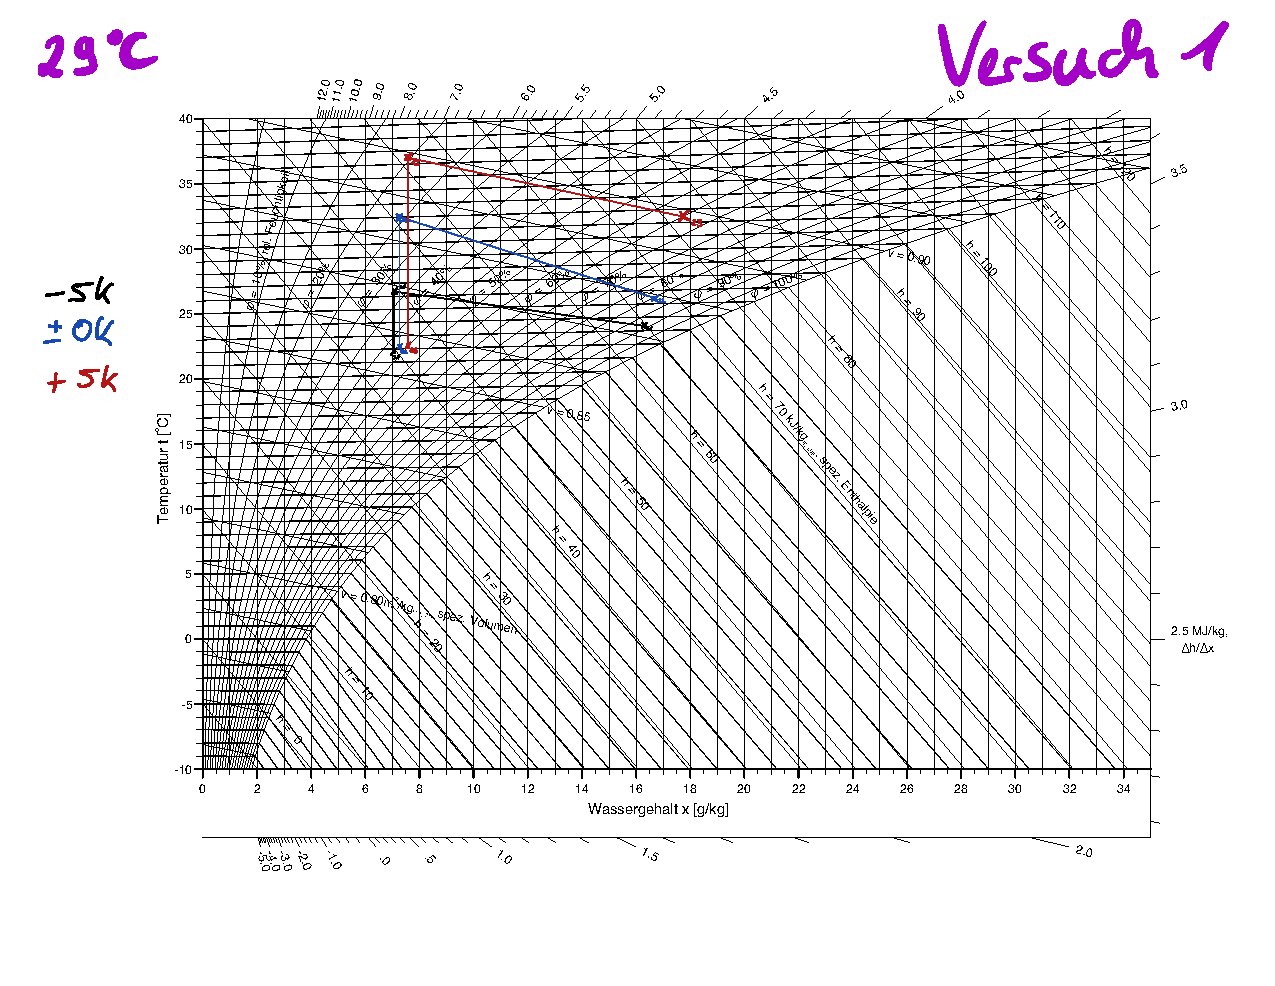
\includepdf[pages=1-3, landscape]{img/hx}

\subsection*{Beispielrechnung eines Datensatzes}
Im folgenden Abschnitt wird eine Berechnung des Volumenstroms für eine Datenreihe mit Hilfe der Theorie aus Abschnitt \ref{sec:physik} durchgeführt.

\begin{flalign}
	\dot{Q}_V &= \dot{m}_{\ce{H2O}}*c_{P_{\ce{H2O}}}*\left(T_{\alpha, \ce{H2O},V}-T_{\omega, \ce{H2O},V}\right)\\
	&= \dot{V}_{\ce{H2O}}*\rho_{\ce{H2O}, \SI{15}{\celsius}}*c_{P_{\ce{H2O}}}*\left(T_{\alpha, \ce{H2O},V}-T_{\omega, \ce{H2O},V}\right)\\
	&= \SI{0,105}{\kmeter \per \hour}*\SI{999,1}{\kg\per \kmeter}*\SI{4,18}{\kilo \joule \per \kelvin \per \kg}*\left(\SI{302,7}{\celsius}-\SI{301,8}{\celsius}\right)\si{\kelvin}\\
	&=\SI{394,7}{\kilo \joule \per \hour} = \SI{0,1096}{\kilo \joule \per \second}\\
	&=\underline{\SI{109,6}{\watt}}
\end{flalign}

\begin{flalign}
	\dot{Q}_{\text{Nutz}}  	&= \dot{m}_{\ce{H2O}}*c_{P_{\ce{H2O}}}*\left(\Delta T_{\ce{H2O},\text{ges}}-\Delta T_{\ce{H2O},V}\right)\\
	\Delta T_{\ce{H2O},\text{ges}}&=\SI{304,4}{\kelvin}-\SI{293,7}{\kelvin} = \SI{10,7}{\kelvin}\\
	\Delta T_{\ce{H2O},V} &=\SI{302,7}{\kelvin}-\SI{301,8}{\kelvin} = \SI{0,9}{\kelvin}\\
	\dot{Q}_{\text{Nutz}}  &= \SI{0,105}{\kmeter \per \hour}*\SI{999,1}{\kg\per \kmeter}*\SI{4,18}{\kilo \joule \per \kelvin \per \kg}*\left(10,7-0,9\right)\si{\kelvin}\\
	&= \SI{4297,3}{\kilo \joule \per \hour} =\SI{1,1937}{\kilo \joule \per \second}\\
	&= \underline{\SI{1193,7}{\watt}}
\end{flalign} 

\begin{flalign}
	%Masse Luft berechenen
\end{flalign}


	
	\begin{landscape}
			\begin{table}[h!]
			\renewcommand*{\arraystretch}{1.2}
			\centering
			%\rowcolors{2}{white}{gray!25}
			\caption{Versuchsreihe 1}
			\label{tab:versuchsreihe1}
			\resizebox{25cm}{!}{
				\begin{tabular}{l|c|c|c|c|c|c|c|c|c|c|c|c|c|c|c|c}
					\hline
					\multicolumn{17}{c}{\textbf{Leitungsverluste}}\\
					\hline
					Temperatur Eingang & \si{\celsius}    &       & \multicolumn{1}{c|}{29,2} &       &       &       &       &       &       &       &       &       &       & \multicolumn{1}{c|}{Dichte für T Ein} & \si{\kg\per\kmeter} & \multicolumn{1}{c}{995,9} \\
					Temperatur Ausgang & \si{\celsius}    &       & \multicolumn{1}{c|}{28,3} &       &       &       &       &       &       &       &       &       &       & \multicolumn{1}{c|}{Volumenstrom} & \si{\liter \per \hour}   & \multicolumn{1}{c}{105,3} \\
					Temperatur Differenz & \si{\celsius}    &       & \multicolumn{1}{c|}{0,9} &       &       &       &       &       &       &       &       &       &       & \multicolumn{1}{c|}{Massestrom} & \si{\kg\per\second}  & \multicolumn{1}{c}{0,029} \\
					Volumenstrom (für 15\si{\celsius}) & \si{\liter \per \hour}   &       & \multicolumn{1}{c|}{105,0} &       &       &       &       &       &       &       &       &       &       & \multicolumn{1}{c|}{Wärmeverlust Leitung } & W     & \multicolumn{1}{c}{109,6} \\
					Dichte (für 15\si{\celsius}) & \si{\kg\per\kmeter} &       & \multicolumn{1}{c|}{999,1} &       &       &       &       &       &       &       &       &       &       &       &       &  \\
					\hline
					&       & \multicolumn{15}{c}{\textit{-5 K, 0 K, +5 K}} \\
					\hline
					&       & \multicolumn{3}{c|}{Lufteingang} & \multicolumn{3}{c|}{Mischluft} & \multicolumn{3}{c|}{Luftausgang} & \multicolumn{3}{c|}{Wassereingang} & \multicolumn{3}{c}{Wasserausgang} \\
					\hline
					Temperatur & \si{\celsius}    & 
					\multicolumn{1}{c|}{21,9} & \multicolumn{1}{c|}{22,1} & \multicolumn{1}{c|}{22,3} &26,3  & 32,0  & 36,80 
					&23,62 & 25,18 & 26,44 
					&\multicolumn{1}{c|}{30,9} & \multicolumn{1}{c|}{30,6} & \multicolumn{1}{c|}{30,8} 
					&\multicolumn{1}{c|}{20,2} & \multicolumn{1}{c|}{21,3} & \multicolumn{1}{c}{22,4} \\
					%
					relative Luftfeuchte & \%    & \multicolumn{1}{c|}{44} & \multicolumn{1}{c|}{44,1} &
					\multicolumn{1}{c|}{44,8} 
					& 33,8  & 24,6  & 19,40 
					& 88,2  & 82,2  & 81,1  & -     & -     & -     & -     & -     & - \\
					absolute Luftfeuchte & \si{\gram \per \kg}  
					& \multicolumn{1}{c|}{7,2} & \multicolumn{1}{c|}{7,3} & \multicolumn{1}{c|}{7,5} 
					& 7,2   & 7,3   & 7,50  
					& 16,2  & 16,6  & 17,7 & -     & -     & -     & -     & -     & - \\
					Enthalpie & \si{\kilo \joule \per \kg} & \multicolumn{1}{c|}{40,4} & \multicolumn{1}{c|}{40,7} & \multicolumn{1}{c|}{41,5} 
					& 44,9  & 50,9  & 56,4  
					& 65,1  & 67,7  & 71,7  & -     & -     & -     & -     & -     & - \\
					\hline
					Temperaturdifferenz  Wasser & K     & -     & -     & -     & \multicolumn{1}{c|}{-} & \multicolumn{1}{c|}{-} & \multicolumn{1}{c|}{-} & \multicolumn{1}{c|}{-} & \multicolumn{1}{c|}{-} & \multicolumn{1}{c|}{-} 
					%
					& \multicolumn{1}{c|}{14,9} & \multicolumn{1}{c|}{9,3} & \multicolumn{1}{c|}{8,4}
					& \multicolumn{1}{c|}{10,7} & 9,3   & 8,4 \\
					%
					Wärmekapazität & \si{\kilo \joule \per \kg \per \kelvin} & -     & -     & -     & \multicolumn{1}{c|}{-} & \multicolumn{1}{c|}{-} & \multicolumn{1}{c|}{-} & \multicolumn{1}{c|}{-} & \multicolumn{1}{c|}{-} & \multicolumn{1}{c|}{-}
					& \multicolumn{1}{c|}{4,18} & \multicolumn{1}{c|}{4,18} & \multicolumn{1}{c|}{4,18} & \multicolumn{1}{c|}{4,18} & 4,18  & 4,18 \\
					Wärmeabgabe Wasser & W     & -     & -     & -     & \multicolumn{1}{c|}{-} & \multicolumn{1}{c|}{-} & \multicolumn{1}{c|}{-} & \multicolumn{1}{c|}{-} & \multicolumn{1}{c|}{-} & \multicolumn{1}{c|}{-} & \multicolumn{1}{c|}{1303,4} & \multicolumn{1}{c|}{1132,8} & \multicolumn{1}{c|}{1023,2} & \multicolumn{1}{c|}{1303,4} & 1132,8 & 1023,2 \\
					Nutzwärme Wasser & W     & -     & -     & -     & \multicolumn{1}{c|}{-} & \multicolumn{1}{c|}{-} & \multicolumn{1}{c|}{-} & \multicolumn{1}{c|}{-} & \multicolumn{1}{c|}{-} & \multicolumn{1}{c|}{-} & \multicolumn{1}{c|}{1193,7} & \multicolumn{1}{c|}{1023,2} & \multicolumn{1}{c|}{913,6} & \multicolumn{1}{c|}{1193,7} & 1023,2 & 913,6 \\
					\hline
					Sättigungsdampfdruck & Pa    & -     & -     & -     & 3413,3 & 4745,0 & 6197,2 & 2909,4 & 3194,1 & 3441,6 & -     & -     & -     & -     & -     & - \\
					universelle Gaskonstante & \si{\joule \per \kg \per \kelvin} & -     & -     & -     & 288,3 & 288,3 & 288,4 & 289,8 & 289,9 & 290,1 & -     & -     & -     & -     & -     & - \\
					\hline
					Dichte & \si{\kg\per\kmeter} & -     & -     & -     & \multicolumn{1}{c|}{1,17} & \multicolumn{1}{c|}{1,15} & 1,13  & \multicolumn{1}{c|}{1,18} & \multicolumn{1}{c|}{1,17} & \multicolumn{1}{c|}{1,17} & \multicolumn{6}{c}{995,9} \\
					\hline
					Massenstrom & \si{\kg\per\second}  &     \multicolumn{9}{|c|}{0,06}    & \multicolumn{6}{c}{0,029} \\
					\hline
					Volumenstrom & \si{\kmeter \per \hour} & -     & -     & -     & 181   & 190   & 190   & 181   & 187   & 184   & \multicolumn{6}{c}{105,3} \\
				\end{tabular}
			}
		\end{table}%
		\FloatBarrier
	\end{landscape}


\begin{landscape}
		\begin{table}[h!]
		\renewcommand*{\arraystretch}{1.2}
		\centering
		%\rowcolors{2}{white}{gray!25}
		\caption{Versuchsreihe 2}
		\label{tab:versuchsreihe2}
		\resizebox{25cm}{!}{
			\begin{tabular}{l|c|c|c|c|c|c|c|c|c|c|c|c|c|c|c|c}
				\hline
				\multicolumn{17}{c}{\textbf{Leitungsverluste}}\\
				\hline
				Temperatur Eingang & \si{\celsius}    &       & \multicolumn{1}{c|}{37,8} &       &       &       &       &       &       &       &       &       &       & \multicolumn{1}{c|}{Dichte für T Ein} & \si{\kg\per\kmeter} & \multicolumn{1}{c}{995,9} \\
				Temperatur Ausgang & \si{\celsius}    &       & \multicolumn{1}{c|}{36,7} &       &       &       &       &       &       &       &       &       &       & \multicolumn{1}{c|}{Volumenstrom} & \si{\liter \per \hour}   & \multicolumn{1}{c}{105,3} \\
				Temperatur Differenz & \si{\celsius}    &       & \multicolumn{1}{c|}{1,1} &       &       &       &       &       &       &       &       &       &       & \multicolumn{1}{c|}{Massestrom} & \si{\kg\per\second}  & \multicolumn{1}{c}{0,029} \\
				Volumenstrom (für 15\si{\celsius}) & \si{\liter \per \hour}   &       & \multicolumn{1}{c|}{105,0} &       &       &       &       &       &       &       &       &       &       & \multicolumn{1}{c|}{Wärmeverlust Leitung } & W     & \multicolumn{1}{c}{134,0} \\
				Dichte (für 15\si{\celsius}) & \si{\kg\per\kmeter} &       & \multicolumn{1}{c|}{999,1} &       &       &       &       &       &       &       &       &       &       &       &       &  \\
				\hline
				&       & \multicolumn{15}{c}{\textit{-5 K, 0 K, +5 K}} \\
				\hline
				&       & \multicolumn{3}{c|}{Lufteingang} & \multicolumn{3}{c|}{Mischluft} & \multicolumn{3}{c|}{Luftausgang} & \multicolumn{3}{c|}{Wassereingang} & \multicolumn{3}{c}{Wasserausgang} \\
				\hline
				Temperatur & \si{\celsius}    & 
				\multicolumn{1}{c|}{22,5} & \multicolumn{1}{c|}{22,4} & \multicolumn{1}{c|}{22,6} 
				&34,0 &  38,4 & 43,6
				&27,5 & 28,8 & 29,9 
				&\multicolumn{1}{c|}{37,8} & \multicolumn{1}{c|}{37,5} & \multicolumn{1}{c|}{36,8} 
				&\multicolumn{1}{c|}{22,9} & \multicolumn{1}{c|}{23,3} & \multicolumn{1}{c}{24,1} \\
				%
				relative Luftfeuchte & \%    & \multicolumn{1}{c|}{41,3} & \multicolumn{1}{c|}{42,5} &
				\multicolumn{1}{c|}{42,5} 
				& 21,1  & 17,0  & 13,1
				& 86,0  & 82,9  & 78,8  & -     & -     & -     & -     & -     & - \\
				absolute Luftfeuchte & \si{\gram \per \kg}  
				& \multicolumn{1}{c|}{7,0} & \multicolumn{1}{c|}{7,2} & \multicolumn{1}{c|}{7,2} 
				& 7,0   & 7,2   & 7,2
				& 20,1 & 20,8  & 21,1 & -     & -     & -     & -     & -     & - \\
				Enthalpie & \si{\kilo \joule \per \kg} & \multicolumn{1}{c|}{40,4} & \multicolumn{1}{c|}{40,9} & \multicolumn{1}{c|}{41,2} 
				& 52,2  & 57,2 & 62,7
				& 79,0  & 82,2 & 84,3  & -     & -     & -     & -     & -     & - \\
				\hline
				Temperaturdifferenz  Wasser & K     & -     & -     & -     & \multicolumn{1}{c|}{-} & \multicolumn{1}{c|}{-} & \multicolumn{1}{c|}{-} & \multicolumn{1}{c|}{-} & \multicolumn{1}{c|}{-} & \multicolumn{1}{c|}{-} 
				& \multicolumn{1}{c|}{14,9} & \multicolumn{1}{c|}{14,2} & \multicolumn{1}{c|}{8,4}
				& \multicolumn{1}{c|}{14,9} & 14,2   & 8,4 \\
				Wärmekapazität & \si{\kilo \joule \per \kg \per \kelvin} & -     & -     & -     & \multicolumn{1}{c|}{-} & \multicolumn{1}{c|}{-} & \multicolumn{1}{c|}{-} & \multicolumn{1}{c|}{-} & \multicolumn{1}{c|}{-} & \multicolumn{1}{c|}{-}
				& \multicolumn{1}{c|}{4,18} & \multicolumn{1}{c|}{4,18} & \multicolumn{1}{c|}{4,18} & \multicolumn{1}{c|}{4,18} & 4,18  & 4,18 \\
				Wärmeabgabe Wasser & W     & -     & -     & -     & \multicolumn{1}{c|}{-} & \multicolumn{1}{c|}{-} & \multicolumn{1}{c|}{-} & \multicolumn{1}{c|}{-} & \multicolumn{1}{c|}{-} & \multicolumn{1}{c|}{-} & \multicolumn{1}{c|}{1815,0} & \multicolumn{1}{c|}{1729,7} & \multicolumn{1}{c|}{1023,2} & \multicolumn{1}{c|}{1815,0} & 1729,7 & 1023,2 \\
				Nutzwärme Wasser & W     & -     & -     & -     & \multicolumn{1}{c|}{-} & \multicolumn{1}{c|}{-} & \multicolumn{1}{c|}{-} & \multicolumn{1}{c|}{-} & \multicolumn{1}{c|}{-} & \multicolumn{1}{c|}{-} & \multicolumn{1}{c|}{1681,0} & \multicolumn{1}{c|}{1595,7} & \multicolumn{1}{c|}{889,2} & \multicolumn{1}{c|}{1681,0} & 1595,7 & 889,2 \\
				\hline
				Sättigungsdampfdruck & Pa    & -     & -     & -     & 5309,4 & 6760,4 & 6197,2 & 3471,2 & 3948,3 & 3441,6 & -     & -     & -     & -     & -     & - \\
				universelle Gaskonstante & \si{\joule \per \kg \per \kelvin} & -     & -     & -     & 288,3 & 288,3 & 288,4 & 290,5 & 290,6 & 290,1 & -     & -     & -     & -     & -     & - \\
				\hline
				Dichte & \si{\kg\per\kmeter} & -     & -     & -     & \multicolumn{1}{c|}{1,14} & \multicolumn{1}{c|}{1,13} & 1,13  & \multicolumn{1}{c|}{1,16} & \multicolumn{1}{c|}{1,15} & \multicolumn{1}{c|}{1,17} & \multicolumn{6}{c}{995,9} \\
				\hline
				Massenstrom & \si{\kg\per\second}  &    0,06&0,06&0,04 &0,06&0,06&0,04  &0,06&0,06&0,04   & \multicolumn{6}{c}{0,029} \\
				\hline
				Volumenstrom & \si{\kmeter \per \hour} & -     & -     & -     & 197   & 204   & 131   & 195   & 199   & 127   & \multicolumn{6}{c}{105,3} \\
			\end{tabular}
		}
	\end{table}%
	\FloatBarrier
\end{landscape}




\begin{landscape}
		\begin{table}[h!]
		\renewcommand*{\arraystretch}{1.2}
		\centering
		%\rowcolors{2}{white}{gray!25}
		\caption{Versuchsreihe 3}
		\label{tab:versuchsreihe3}
		\resizebox{25cm}{!}{
			\begin{tabular}{l|c|c|c|c|c|c|c|c|c|c|c|c|c|c|c|c}
				\hline
				\multicolumn{17}{c}{\textbf{Leitungsverluste}}\\
				\hline
				Temperatur Eingang & \si{\celsius}    &       & \multicolumn{1}{c|}{42,6} &       &       &       &       &       &       &       &       &       &       & \multicolumn{1}{c|}{Dichte für T Ein} & \si{\kg\per\kmeter} & \multicolumn{1}{c}{995,9} \\
				Temperatur Ausgang & \si{\celsius}    &       & \multicolumn{1}{c|}{40,6} &       &       &       &       &       &       &       &       &       &       & \multicolumn{1}{c|}{Volumenstrom} & \si{\liter \per \hour}   & \multicolumn{1}{c}{105,3} \\
				Temperatur Differenz & \si{\celsius}    &       & \multicolumn{1}{c|}{2,0} &       &       &       &       &       &       &       &       &       &       & \multicolumn{1}{c|}{Massestrom} & \si{\kg\per\second}  & \multicolumn{1}{c}{0,029} \\
				Volumenstrom (für 15\si{\celsius}) & \si{\liter \per \hour}   &       & \multicolumn{1}{c|}{105,0} &       &       &       &       &       &       &       &       &       &       & \multicolumn{1}{c|}{Wärmeverlust Leitung } & W     & \multicolumn{1}{c}{243,6} \\
				Dichte (für 15\si{\celsius}) & \si{\kg\per\kmeter} &       & \multicolumn{1}{c|}{999,1} &       &       &       &       &       &       &       &       &       &       &       &       &  \\
				\hline
				&       & \multicolumn{15}{c}{\textit{-5 K, 0 K, +5 K}} \\
				\hline
				&       & \multicolumn{3}{c|}{Lufteingang} & \multicolumn{3}{c|}{Mischluft} & \multicolumn{3}{c|}{Luftausgang} & \multicolumn{3}{c|}{Wassereingang} & \multicolumn{3}{c}{Wasserausgang} \\
				\hline
				Temperatur & \si{\celsius}    & 
				\multicolumn{1}{c|}{22,3} & \multicolumn{1}{c|}{22,4} & \multicolumn{1}{c|}{22,8} 
				&38,8 &  44,0 & 48,9
				&30,1 & 31,6 & 32,4 
				&\multicolumn{1}{c|}{34,1} & \multicolumn{1}{c|}{42,0} & \multicolumn{1}{c|}{41,9} 
				&\multicolumn{1}{c|}{24,7} & \multicolumn{1}{c|}{25,2} & \multicolumn{1}{c}{27,6} \\
				%
				relative Luftfeuchte & \%    & \multicolumn{1}{c|}{42,8} & \multicolumn{1}{c|}{42,9} &
				\multicolumn{1}{c|}{42,7} 
				& 17,3  & 12,8  & 10,1
				& 87,5  & 83,8  & 80,0  & -     & -     & -     & -     & -     & - \\
				absolute Luftfeuchte & \si{\gram \per \kg}  
				& \multicolumn{1}{c|}{7,4} & \multicolumn{1}{c|}{7,2} & \multicolumn{1}{c|}{7,3} 
				& 7,4   & 7,2   & 7,3
				& 23,8 & 24,8  & 24,8 & -     & -     & -     & -     & -     & - \\
				Enthalpie & \si{\kilo \joule \per \kg} & \multicolumn{1}{c|}{42,0} & \multicolumn{1}{c|}{41,1} & \multicolumn{1}{c|}{41,7} 
				& 58,3  & 63,1 & 68,4
				& 91,3  & 95,4 & 96,2 & -     & -     & -     & -     & -     & - \\
				\hline
				Temperaturdifferenz  Wasser & K     & -     & -     & -     & \multicolumn{1}{c|}{-} & \multicolumn{1}{c|}{-} & \multicolumn{1}{c|}{-} & \multicolumn{1}{c|}{-} & \multicolumn{1}{c|}{-} & \multicolumn{1}{c|}{-} 
				& \multicolumn{1}{c|}{18,4} & \multicolumn{1}{c|}{16,8} & \multicolumn{1}{c|}{14,3}
				& \multicolumn{1}{c|}{18,4} & 16,8   & 14,3\\
				Wärmekapazität & \si{\kilo \joule \per \kg \per \kelvin} & -     & -     & -     & \multicolumn{1}{c|}{-} & \multicolumn{1}{c|}{-} & \multicolumn{1}{c|}{-} & \multicolumn{1}{c|}{-} & \multicolumn{1}{c|}{-} & \multicolumn{1}{c|}{-}
				& \multicolumn{1}{c|}{4,18} & \multicolumn{1}{c|}{4,18} & \multicolumn{1}{c|}{4,18} & \multicolumn{1}{c|}{4,18} & 4,18  & 4,18 \\
				Wärmeabgabe Wasser & W     & -     & -     & -     & \multicolumn{1}{c|}{-} & \multicolumn{1}{c|}{-} & \multicolumn{1}{c|}{-} & \multicolumn{1}{c|}{-} & \multicolumn{1}{c|}{-} & \multicolumn{1}{c|}{-} & \multicolumn{1}{c|}{2241,3} & \multicolumn{1}{c|}{2046,4} & \multicolumn{1}{c|}{1741,9} & \multicolumn{1}{c|}{2241,3} & 2046,4 & 1741,9 \\
				Nutzwärme Wasser & W     & -     & -     & -     & \multicolumn{1}{c|}{-} & \multicolumn{1}{c|}{-} & \multicolumn{1}{c|}{-} & \multicolumn{1}{c|}{-} & \multicolumn{1}{c|}{-} & \multicolumn{1}{c|}{-} & \multicolumn{1}{c|}{1997,7} & \multicolumn{1}{c|}{1802,8} & \multicolumn{1}{c|}{1498,3} & \multicolumn{1}{c|}{1997,7} & 1802,8 & 1498,3 \\
				\hline
				Sättigungsdampfdruck & Pa    & -     & -     & -     & 6907,9 & 9096,3 & 11683,9 & 4260,5 & 4630,8 & 4842,6 & -     & -     & -     & -     & -     & - \\
				universelle Gaskonstante & \si{\joule \per \kg \per \kelvin} & -     & -     & -     & 288,3 & 288,7 & 288,3 & 291,1& 291,2 & 291,3 & -     & -     & -     & -     & -     & - \\
				\hline
				Dichte & \si{\kg\per\kmeter} & -     & -     & -     & \multicolumn{1}{c|}{1,13} & \multicolumn{1}{c|}{1,11} & 1,09  & \multicolumn{1}{c|}{1,15} & \multicolumn{1}{c|}{1,14} & \multicolumn{1}{c|}{1,14} & \multicolumn{6}{c}{995,9} \\
				\hline
				Massenstrom & \si{\kg\per\second}  &   0,06&0,06&0,05 &0,06&0,06&0,05  &0,06&0,06&0,05  & \multicolumn{6}{c}{0,029} \\
				\hline
				Volumenstrom & \si{\kmeter \per \hour} & -     & -     & -     & 193   & 182   & 178   & 190   & 176   & 170   & \multicolumn{6}{c}{105,3} \\
			\end{tabular}
		}
	\end{table}%
	\FloatBarrier
\end{landscape}


